
\documentclass{exam}

\usepackage{graphicx}
\usepackage[fleqn]{amsmath}
\usepackage{unitsdef} 
\usepackage{cancel}
\usepackage{float}
\usepackage{mdwlist}
\usepackage{booktabs}
\usepackage{cancel}
\usepackage{polynom}
\usepackage{caption}
\usepackage{parskip}
\usepackage{fullpage}
\usepackage{enumerate}

% \newcommand{\degree}{\ensuremath{^\circ}} 
\everymath{\displaystyle}

\newunit{\inch}{in}
\newunit{\foot}{ft}
\newunit{\cemtimeter}{cm}

% \begin{figure}[H]
%   \centering
%   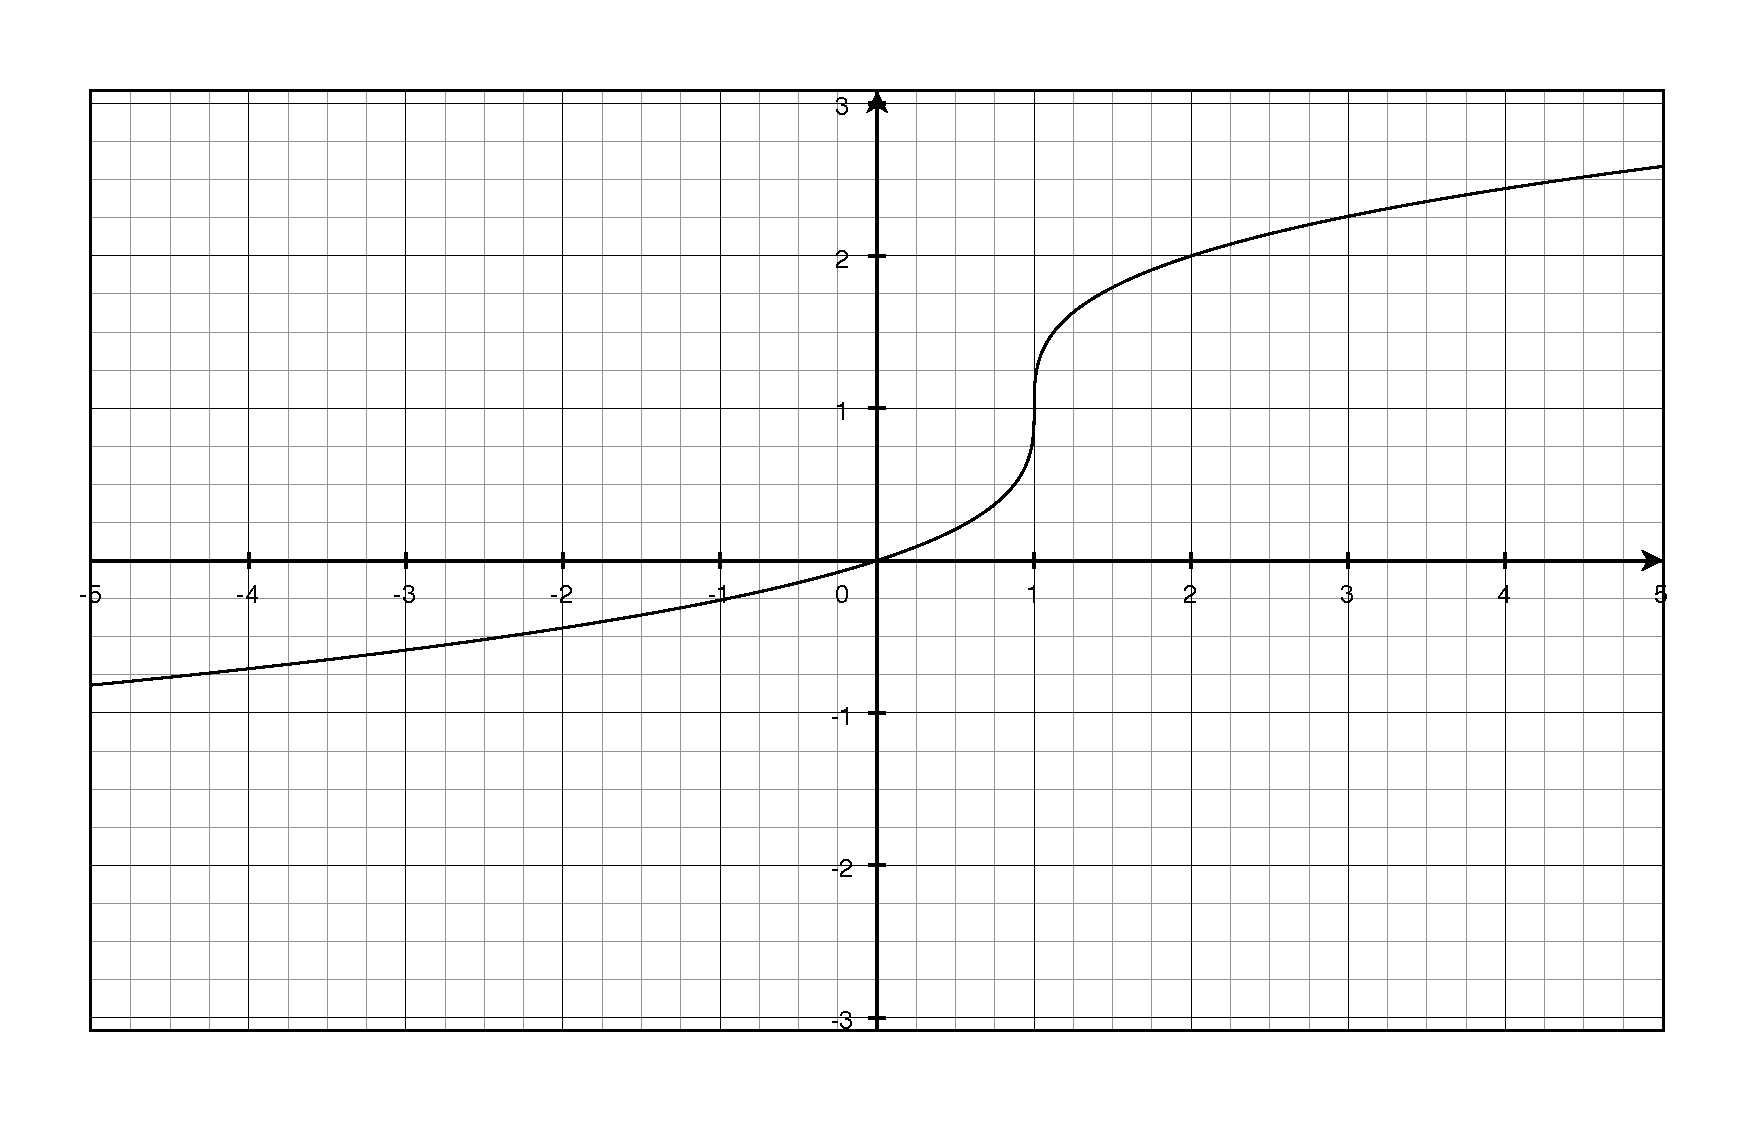
\includegraphics[scale=.3]{question7.eps}
%   \caption*{Question 7}
% \end{figure}

% \begin{tabular}{cc}
% \toprule
% period & amplitude \\
% \midrule
%   $\pi$ & $2$ \\
% \bottomrule
% \end{tabular}

\printanswers

\ifprintanswers 
\usepackage{2in1, lscape} 
\fi

\title{Math 263B \\ Homework Nine \\ Exponential and Logarithm Review}
\date{September 20, 2012}

\begin{document}

\maketitle

\ifprintanswers
\else

\section{Notes}

\subsection{Logarithm Definition}

If $x = b^y$ then $y = \log_b x$.  $y$ is the number you need to raise $b$ to to get $x$.

$e \approx 2.71828182846$ is the base of the {\em natural logarithm} ($\ln$).  $e$ is used for  computing compound interest and
is also useful in calculus.

\subsection{Logarithm Facts}

\begin{itemize}
  \item $\log_a 1 = 0$ because $a^0 = 1$
  \item $\log_a a = 1$ because $a^1 = a$
  \item $\log_a a^x = x$ 
  \item $a^{\log_a x} = x$ 
  \item $\log_a x = \frac{\log_b x}{\log_b a}$
  \item $\log_a (uv) = \log_a u + \log_a v$
  \item $\log_a \left(\frac{u}{v} \right) = \log_a u - \log_a v$
  \item $\log_a u^n = n \log_a u$
\end{itemize}

\subsection{Interest}
Given an annual interest rate, the lender ends up with more money the more frequently the interest is compounded.  This is
because you get interest on the interest, interest on the interest on the interest, etc.

If $P$ is the principal, $r$ is the annual rate, $t$ is the number of years, and you have $n$ compondings per year, the 
formula is: $A = P\left( 1 + \frac{r}{n} \right)^{nt}$

The best case, for the lender, is compounding continuously.  This gives you: $A = P e^{rt}$
\fi

\section{Homework}

\begin{questions}

\uplevel{For questions \ref{form:first} to \ref{form:last} write the equation in logarithmic form.  For example, the logarithmic
form of $2^3 = 8$ is $\log_2 8 = 3$.}

\question $5^3 = 125$
\label{form:first}
\begin{solution}
\[
  \log_5 125 = 3
\]
\end{solution}


\question $8^2 = 64$
\begin{solution}
\[
  \log_8 64 = 2
\]
\end{solution}

\question $6^{-2} = \frac{1}{36}$
\begin{solution}
\[
  \log_6 \frac{1}{36} = -2
\]
\end{solution}

\question $9^{3/2} = 27$
\begin{solution}
\[
  \log_9 27 = \frac{3}{2}  
\]
\end{solution}

\question $e^x = 4$
\begin{solution}
\[
  \ln 4 = x
\]
\end{solution}

\label{form:last}

\uplevel{For questions \ref{evaluate:first} to \ref{evaluate:last} evaluate the expression without using a calculator.}

\question $\log_3 81$
\label{evaluate:first}
\begin{solution}
  $\log_3 81 = 4$ because $3^4 = 81$.
\end{solution}

\question $\log_2 16$
\begin{solution}
  $\log_2 16 = 4$ because $2^4 = 16$.
\end{solution}

\ifprintanswers
\pagebreak
\fi

\question $\log_7 1$
\begin{solution}
$\log_7 1 = 0$ because $7^0 = 1$.
\end{solution}

\question $\log_{27} 9$
\begin{solution}
$\log_{27} 9 = \frac{2}{3}$ because $27^{2/3} = 9$.
\end{solution}

\question $\ln e^{-2}$
\label{evaluate:last}
\begin{solution}
$\ln e^{-2} = -2$
\end{solution}

\uplevel{For questions \ref{expand:first} to \ref{expand:last} expand the expression into a sum, difference, and/or
  constant multiple of logarithms.}

\question $\log_{10} 5x$
\label{expand:first}
\begin{solution}
\[
    \log_{10} 5x = \log_{10} 5 + \log_{10} x
\]
\end{solution}

\question $\ln \sqrt{z}$
\begin{solution}
\[
  \ln \sqrt{z} = \ln z^{1/2} = \frac{1}{2} \ln z
\]
\end{solution}

\question $\ln xyz$
\begin{solution}
\[
  \ln xyz = \ln x + \ln y + \ln z  
\]
\end{solution}

\question $\log_b \left( \frac{x^2}{y^2z^3} \right)$
\begin{solution}
\begin{align*}
  \log_b \left( \frac{x^2}{y^2z^3} \right) &= \log_b x^2 - \log_b y^2z^2 \\
  &= 2 \log_b x - \left( \log_b y^2 + \log_b z^3 \right) \\
  &= 2 \log_b x - (2 \log_b y + 3 \log_b z) \\
  &= 2 \log_b x - 2 \log_b y - 3 \log_b z \\
\end{align*}

\end{solution}

\question $\ln \sqrt{x^2y^{-1}}$
\label{expand:last}
\begin{solution}

approach one:
\begin{align*}
  \ln \sqrt{x^2y^{-1}} &= \ln \left(x^2y^{-1} \right)^{1/2} \\
  &= \ln xy^{-1/2} \\
  &= \ln x - \frac{1}{2} \ln y \\
\end{align*}

approach two:
\begin{align*}
  \ln \sqrt{x^2y^{-1}} &= \ln \left(x^2y^{-1} \right)^{1/2} \\
  &= \frac{1}{2} \ln \left( x^2 y^{-1} \right) \\
  &= \frac{1}{2} \left( \ln x^2 + \ln y^{-1} \right) \\
  &= \frac{1}{2} \left( 2 \ln x - \ln y \right) \\
  &= \ln x - \frac{1}{2} \ln y \\
\end{align*}

\end{solution}

\uplevel{For questions \ref{condense:first} to \ref{condense:last} condense the expression into a logarithm of a single quantity.}

\question $\ln x + \ln 3$
\label{condense:first}
\begin{solution}
\[
  \ln x + \ln 3 = \ln 3x
\]
\end{solution}

\question $3 \log_2(x + 4)$
\begin{solution}
\[
  3 \log_2(x + 4) = \log_2 (x + 4)^3
\]
\end{solution}

\question $3 \ln x + 4 \ln y - 2 \ln z$
\begin{solution}
\begin{align*}
  3 \ln x + 4 \ln y - 2 \ln z &= \ln x^3 + \ln y^4 - \ln z^2 \\
  &= \ln \frac{x^3y^4}{z^2} \\
\end{align*}
\end{solution}

\question $2 \ln 3 - \frac{1}{2} \ln \left(x^2 + 1 \right)$
\begin{solution}
\begin{align*}
  2 \ln 3 - \frac{1}{2} \ln \left(x^2 + 1 \right) &= \ln 3^2 - \ln \left( x^2 + 1 \right)^{1/2} \\
  &= \ln \frac{9}{\sqrt{x^2 + 1}} \\
\end{align*}

\end{solution}

\question $2[ \ln x - \ln(x + 1) - \ln(x - 1)]$
\label{condense:last}

\begin{solution}
\begin{align*}
  2[ \ln x &- \ln(x + 1) - \ln(x - 1)] \\
  &= 2 \ln \left( \frac{x}{(x+1)(x-1)} \right) \\
  &= 2 \ln \left( \frac{x}{x^2-1} \right) \\
  &= \ln \left( \frac{x}{x^2-1} \right)^2 \\
\end{align*}
\end{solution}

\pagebreak

\uplevel{For questions \ref{base:first} to \ref{base:last} use the change-of-base formula to convert the logarithm to
  base 10 logarthim and evaulate using a calculator.}

\question $\log_3 7$
\label{base:first}
\begin{solution}
\[
  \log_3 7 = \frac{\log 7}{\log 3} \approx 1.7712
\]
\end{solution}

\question $\log_7 4$
\label{base:last}
\begin{solution}
\[
  \log_7 4 = \frac{\log 4}{\log 7} \approx 0.7124
\]
\end{solution}

\question
With a principal of 1,000 and an interest rate of 5\%, how much money do you have after 10 years if the interest is
compounded:
\begin{parts}
\part annually
\begin{solution}
\[
  A = \$ 1,000(1 + 0.05)^{10} = \$ 1,628.89
\]
\end{solution}

\part monthly
\begin{solution}
\[
  A = \$ 1,000 \left(1 + \frac{0.05}{12} \right)^{10 \cdot 12} = \$ 1,647.01
\]
\end{solution}

\ifprintanswers
\pagebreak
\fi

\part daily
\begin{solution}
\[
  A = \$ 1,000 \left(1 + \frac{0.05}{365} \right)^{10 \cdot 365} = \$ 1,648.66
\]
\end{solution}

\part continuously
\begin{solution}
\[
  A = \$ 1,000 e^{.05 \cdot 10} = \$ 1,648.72
\]
\end{solution}

\end{parts}

\end{questions}

%% \ifprintanswers
%% \pagebreak
%% \fi

\ifprintanswers
\else

\vspace{14 cm}

I don't believe in any form of unjustified extremism. But when a man is exercising extremism---a human being is
exercising extremism---in defense of liberty for human beings it's no vice, and when one is moderate in the pursuit of
justice for human beings I say he is a sinner.

\hspace{0.5 cm} 
--Malcolm X

%% {\em Some writers have so confounded society with government, as to leave little or no distinction between them; whereas
%%   they are not only different, but have different origins. Society is produced by our wants, and government by our
%%   wickedness; the former promotes our happiness POSITIVELY by uniting our affections, the latter NEGATIVELY by
%%   restraining our vices. The one encourages intercourse, the other creates distinctions. The first a patron, the last a
%%   punisher.} --Thomas Paine

\fi

\end{document}

